\documentclass[atmosphere,article,accept,pdftex,moreauthors]{Definitions/mdpi}

% %%
% MDPI internal commands - do not modify
\firstpage{1}
\makeatletter
\setcounter{page}{\@firstpage}
\makeatother
\pubvolume{1}
\issuenum{1}
\articlenumber{0}
\pubyear{2024}
\copyrightyear{2024}
\externaleditor{Academic Editor:  Abd Al Karim Haj Ismail}
\datereceived{21 December 2023 }
\daterevised{1 February 2024 } % Comment out if no revised date
\dateaccepted{7 February 2024 }
\datepublished{ }
%\datecorrected{} % For corrected papers: "Corrected: XXX" date in the original paper.
%\dateretracted{} % For corrected papers: "Retracted: XXX" date in the original paper.
\hreflink{https://doi.org/} % If needed use \linebreak
%\doinum{}
%\pdfoutput=1 % Uncommented for upload to arXiv.org

% %% title page
% Full title of the paper (Capitalized)
\Title{
	Gridded Assessment of Mainland China's Solar Energy Resources using the Typical Meteorological Year Method and China Meteorological Forcing Dataset
	}

% MDPI internal command: TbTitle for citation in the left column
\TitleCitation{Gridded Assessment of Mainland China's Solar Energy Resources using the Typical Meteorological Year Method and China Meteorological Forcing Dataset}

% Author Orchid ID: enter ID or remove command
\newcommand{\orcidauthorS}{0000-0002-1331-002X}
\newcommand{\orcidauthorZ}{0000-0001-7580-9128}

% Authors, for the paper (add full first names)
\Author{Zongpeng Song \textsuperscript{1}\orcidS{}, Bo Wang \textsuperscript{1}, Hui Zheng \textsuperscript{2,}*\orcidZ{}, Shuanglong Jin \textsuperscript{1}, Xiaolin Liu \textsuperscript{1} and Shenbing Hua \textsuperscript{1}}

%\longauthorlist{yes}

% MDPI internal command: Authors, for metadata in PDF
\AuthorNames{Zongpeng Song, Bo Wang, Hui Zheng, Shuanglong Jin, Xiaolin Liu, and Shenbing Hua}

% MDPI internal command: Authors, for citation in the left column
\AuthorCitation{Song, Z.; Wang, B.; Zheng, H.; Jin S.; Liu, X.; Hua, S.}

% Affiliations / Addresses (Add [1] after \address if there is only one affiliation.)
\address{%
$^{1}$ \quad National Key Laboratory of Renewable Energy Grid-Integration, China Electric Power Research Institute, Beijing 100192, China; songzongpeng@epri.sgcc.com.cn (Z.S.); wangbo@epri.sgcc.com.cn (B.W.); jinshuanglong@epri.sgcc.com.cn (S.J.); liuxiaolin@epri.sgcc.com.cn (X.L.); \mbox{huashenbing@epri.sgcc.com.cn (S.H.)}\\
$^{2}$ \quad Key Laboratory of Regional Climate-Environment Research for Temperate East Asia, Institute of Atmospheric Physics, Chinese Academy of Sciences, Beijing 100029, China}

% Contact information of the corresponding author
\corres{Correspondence: zhenghui@tea.ac.cn}

%\simplesumm{} % Simple summary

% %% Abstract (Do not insert blank lines, i.e. \\)
\abstract{
    The National Standard of China has recommended the typical meteorological year (TMY) method for assessing solar energy resources. Compared with the widely adopted multi-year averaging (MYA) methods, the TMY method can consider the year-to-year variations of weather conditions and characterize solar radiation under climatological weather conditions. However, there are very few TMY-based solar energy assessments on the scale of China. On the national scale, the difference between the TMY and MYA methods, the requirement of the data record length, and the impacts of the selection of meteorological variables on the TMY-based assessment are still unclear. This study aims to fill these gaps by assessing mainland China's solar energy resources using the TMY method and China Meteorological Forcing Dataset. The results show that the data record length could significantly influence annual total solar radiation estimation when the record length is shorter than 30 years. Whereas, the estimation becomes stable when the length is greater or equal to 30 years, suggesting a thirty-year data record is preferred. The difference between the MYA and TMY methods is exhibited primarily in places with modest or low abundance of solar radiation. The difference is nearly independent of the examined data record lengths, hinting at the role of regional-specific weather characteristics. The TMY and MYA methods differ more pronounced when assessing the seasonal stability grade. A total of 7.4\% of the area of China experiences a downgrade from the TMY relative to the MYA methods, while a 3.15\% area experiences an upgrade. The selection of the meteorological variables has a notable impact on the TMY-based assessment. Among the three meteorological variables examined, wind speed has the most considerable impact on both the annual total and seasonal stability, dew point has the second most significant impact, and air temperature has the least. The results are useful for guiding future research on solar energy assessment in China and could be helpful for solar energy development planning.
	}

% %% Keywords
\keyword{solar energy abundance; typical meteorological year; seasonal stability index; reference period length}

\begin{document}
% %% Introduction
\section{Introduction}\label{sec:intro}

Solar energy is abundant, clean, and~widely distributed. It is an important renewable energy source for decarbonizing the energy system. However, solar energy varies significantly in space and time~\cite{wang2015JGRA, he2020GRLa, shaner2018EES}. Assessing the abundance and stability of solar energy resources on a national scale at a fine spatial resolution is essential for renewable energy development planning~\cite{shaner2018EES, tong2021NC}.

Plenty of studies have assessed the solar energy resources of China. To name a few, Tang~et~al.~\cite{tang2023JCP} compiled a set of high-accuracy in situ solar radiation observations and assessed the technical potential for solar photovoltaic generation in China. Shi~et~al.~\cite{shi2023RSER} retrieved the solar photovoltaic map of China using the Fengyun-4 geostationary satellite observations. Despite the differences in the data sources, these assessment depends on solely solar radiation data and calculate the solar energy resources as multi-year averages (MYA) of the~data.

It has been well recognized that the variation of solar energy is predominantly due to weather conditions. Since weather systems have nonlinear impacts on surface solar radiation, the~arithmetic average of solar radiation differs from that under representative weather conditions~\cite{abreu2018RE}. The~typical meteorological year (TMY) method aims to address this issue, as~shown in \Cref{tab:cmp}. The~method consists of two steps: generation of a TMY that could characterize the representative weather conditions and assessment of solar energy resources based on the generated TMY~\cite{li2020E, abreu2018RE, chang2017PM, jiang2010E, bulut2004RE, kambezidis2020TAC, markou2007AE, pissimanis1988SE}.

\begin{table}[H]

  \caption{Comparison between the MYA and TMY~methods.\label{tab:cmp}}
  \begin{adjustwidth}{-4.6cm}{0cm}
    \newcolumntype{C}{>{\centering\arraybackslash}X}
    \begin{tabularx}{\fulllength}{CCC}
      \toprule
      \textbf{Aspect}                                     & \textbf{MYA}                                                        & \textbf{TMY}                                                                                                          \\
      \midrule
      Input data                                          & Use solar radiation data only.                                      & Use solar radiation and multiple surface meteorological variables such as air temperature, wind speed, and~dew~point. \\
      \midrule
      Calculation of annual solar radiation               & Arithmetic average of the solar radiation data over multiple years. & Arithmetic average of the solar radiation over a TMY. The~TMY is generated using multiple meteorological~variables.   \\
      \midrule
      Calculation of annual solar \mbox{radiation cycle.} & Multi-year averaged annual cycle                                    & Annual cycle of the~TMY.
      \\  \midrule
      Consideration of extreme \mbox{weather conditions}  & No.                                                                 & Yes. Consider the climatology of extreme daily statistics such as maximum and minimum air~temperature.                \\
      \bottomrule
    \end{tabularx}
  \end{adjustwidth}
\end{table}

The TMY method originates at the Sandia National Laboratories~\cite{hall1978}. A~TMY is a set of 12 months. Each month is selected from a set of multiple years in a place. The~weather characteristics of each month are closest to the climatology of the site. The~closeness of the weather is measured by the weighted average of the Finkelstein--Schafer statistics of multiple meteorological variables. The~variables often include solar radiation, wind speed, air temperature, and~dew point. Since its origin, the~TMY method has an increasing number of variations~\cite{janjai2009AE, ecevit2002E, petrie1978SE, feuermann1985SE, al-hinai1995AE, mosalamshaltout1994RE}. While the variations make no difference in the use of the Finkelstein--Schafer statistics, they differ mainly in the considered meteorological variables and the weights in averaging the variables. The~Sandia, Danish, and~Festa--Ratto approaches are three widely adopted variations. The~Sandia approach employs nine daily statistics of four meteorological variables: (1) the daily mean, maximum, and~minimum air temperature; (2) the daily mean, maximum, and~minimum air humidity; (3) the daily mean and maximum wind speed, and;~(4) the daily mean global solar radiation~\cite{hall1978, kambezidis2020TAC, markou2007AE, pissimanis1988SE, argiriou1999SE}. The~Danish approach uses seven daily statistics of six variables, including daily maximum and mean air temperature, mean relative humidity, mean wind speed, mean atmospheric pressure, sunshine duration, and~global radiation~\cite{argiriou1999SE}. The~Danish approach also removes the seasonal cycle from air temperature and global radiation and normalizes the daily residuals with their respective standard deviation. The~Festa--Ratto approach~\cite{festa1993SE} uses five daily statistics of four variables, which are daily maximum and mean temperature, mean relative humidity, mean wind speed, and~global radiation. Similar to the Danish approach, the~Festa--Ratto approach removes the smoothed long-term monthly mean from the daily variables and normalizes the daily residuals using the standard deviation. Due to its simplicity, the~Sandia approach is still the most widely used~one.

The National Standard of China (GB/T~42766--2023)~\cite{GBT42766-2023} has recommended the Sandia TMY method with slight modifications~\cite{chang2017PM}. The~method has been widely adopted for plot-scale assessment in various climate regimes~\cite{chang2017PM, polo2020E, jiang2010E, zhou2006RE}. However, studies on the scale of China are few. To~our knowledge, Solargis may be the only assessment product yet~\cite{cebecauer2015EP}. TMYs are created using the European Centre for Medium-Range Weather Forecasts Reanalysis version 5 (ERA5)~\cite{hersbach2020QJRMS, bell2021QJRMS} and Integrated Forecast System (IFS) data. It is a commercial product (\url{https://solargis.com} (accessed on 20 December 2023)), and~the details of the production methods are largely not~disclosed.

Due to the inadequacy of published studies, several scientific questions remain unclear in the national-scale solar energy assessment: how is the TMY method compared with the MYA method; what is the requirement of the data record length (in other words, the~length of the reference climatology); and what is the impact of the included meteorological variables on the~assessment.

This study aims to answer these questions by providing a gridded assessment using the TMY method and the China Meteorological Forcing Dataset (CMFD) version 1.7~\cite{he2020SD}. The~dataset is based on ERA5, with~the biases being corrected using in situ observations. The~correction improves the accuracy of the estimation of the meteorological variables~\cite{yang2017HESS, lei2023ESS}. Consequently, CMFD would be more suitable than ERA5 (used by Solargis) in generating TMY for~China.

The paper is organized as follows. \Cref{sec:datamethods} details the TMY method, the~used dataset, the~experimental settings, and~the analysis method. \Cref{sec:results} presents the results and discussion. Finally, \Cref{sec:conclusions} draws the~conclusions.

\section{Data and~Methods}\label{sec:datamethods}
\unskip

\subsection{China Meteorological Forcing~Dataset}\label{sec:datamethods:cmfd}

The CMFD version 1.7~\cite{he2020SD} is a long-term, gridded surface meteorological dataset of mainland China at a spatial resolution of 0.1\textdegree{} and a temporal resolution of 3 hours from 1951 to 2020. The~dataset is created based on ERA5~\cite{hersbach2020QJRMS, bell2021QJRMS}. Biases in the reanalysis are corrected using in situ observations. The~observations are from the China Meteorological Administration (CMA) and the National Oceanic and Atmospheric Administration's National Centers for Environmental Information (NOAA NCEI). Validation against independent observations suggests that the quality is reasonable and consistent across mainland China~\cite{he2020SD, yang2017HESS, lei2023ESS}.

CMFD contains multiple surface meteorological variables, including 10-m wind speed, 2-m air temperature, specific humidity, surface air pressure, downwelling solar irradiance, downwelling longwave irradiance, and~precipitation. These variables are sufficient to characterize the interannual variations of weather conditions while facilitating the TMY-based assessment of solar energy~resources.

\subsection{Typical Meteorological~Year}\label{sec:datamethods:tmy}

We generated TMYs at each CMFD grid cell. \Cref{fig:diagram} shows the diagram of the generation procedure. The~procedure mostly follows the National Standard of China (GB/T~42766-2023)~\cite{GBT42766-2023}.

First, dew point temperature (\(T_\mathrm{d}\); \(\mathrm{K}\)) was calculated from the three-hourly CMFD records by solving the equation of partial water vapor pressure as follows.
\begin{linenomath}
  \begin{equation}
    P_\mathrm{s}(T_\mathrm{d}) = \frac{q p}{\epsilon + (1-\epsilon)q}  \text{,}
  \end{equation}
\end{linenomath}
where \(q\) and \(p\) are the specific humidity (\(\mathrm{kg\,kg^{-1}}\)) and surface air pressure (\(\mathrm{Pa}\)) from the CMFD, respectively. \(\epsilon=0.622\) is the ratio of water vapor's molecular weight to the average dry air molecular weight. \(P_\mathrm{s}(T)\) is the relationship between saturation water-vapor pressure (\(P_\mathrm{s}\); \(\mathrm{Pa}\)) and temperature (\(T\); \(\mathrm{K}\)). The~relationship can be written as follows~\cite{huang2018JAMC}.
\begin{linenomath}
  \begin{equation}
    P_s(T) = \frac{\exp(34.494 - \frac{4924.99}{T - 36.06})}{(T - 168.16)^{1.57}} \text{.}
  \end{equation}
\end{linenomath}

The values of CMFD-specific humidity could occasionally approach zero, leading to an exceptionally low dew point temperature. To~reduce the impact of these abnormal values on the statistics such as the daily mean and minimum, a~minimum dew point temperature was set as \(T_\mathrm{d} \ge -65~\mathrm{^\circ C}\). The~minimum dew point corresponds to the saturated water vapor pressure of \(1.1~\mathrm{Pa}\).

\begin{figure}[H]
  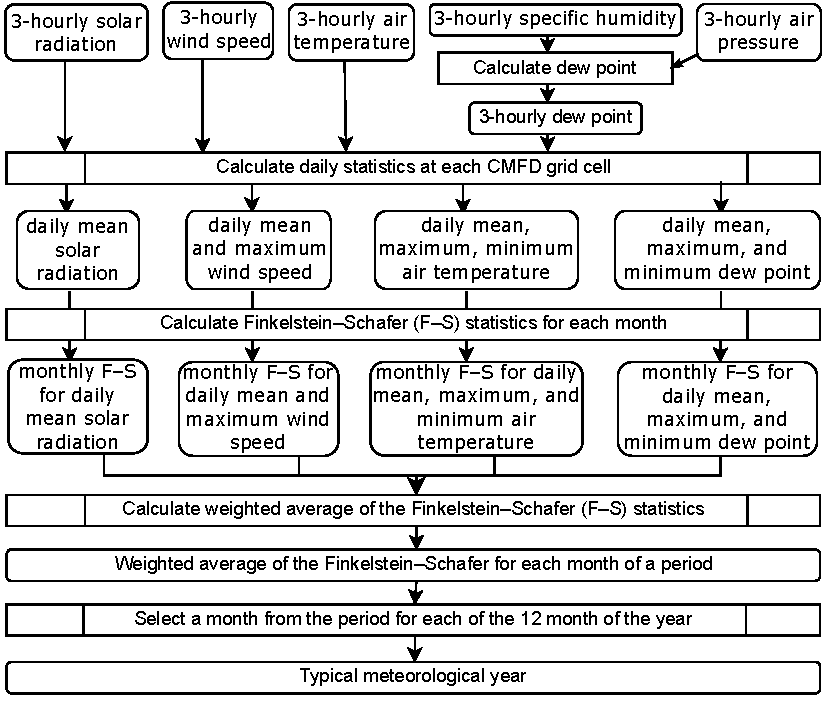
\includegraphics[width=13.8cm]{fig/diagram.pdf}
  \caption{Schematic diagram of the TMY generation procedure. The~five three-hourly variables shown at the top are from~CMFD.\label{fig:diagram}}
\end{figure}

Second, daily statistics (i.e., mean, maximum, and~minimum) were calculated from three-hourly data for four meteorological variables. The~four variables are the surface downwelling solar radiation, 2m air temperature, 10m wind speed, and~dew point temperature. The~first three were obtained directly from the CMFD\@.

Third, given a period that could span multiple years, monthly Finkelstein--Schafer statistic (\(F_{y,m}\))~\cite{finkelstein1971B} was calculated for each month \(m\) and year \(y\) of the period and for each daily statistics \(X\) as follows~\cite{GBT42766-2023}.
\begin{linenomath}
  \begin{equation}
    F_{y,m} = \frac{1}{n_{y,m}} \sum_{i=1}^{n_{y,m}} |S_{y,m}(X_{y,m,i}) - S_m(X_{y,m,i})| \text{,}
  \end{equation}
\end{linenomath}
where \(n_{y,m}\) is the number of days of the month \(m\) and year \(y\), \(X_{y,m,i}\) is the \(i\)-th daily value in ascending~order.

\(S_{y,m}\) is monthly cumulative distribution function for month \(m\) and year \(y\). The~calculation is similar to \Cref{eq:cdf_clim}.
\begin{linenomath}
  \begin{equation}\label{eq:cdf_mon}
    S_{y,m}(X_{y,m,i}) = \frac{i - 0.5}{n_{y,m}} \text{.}
  \end{equation}
\end{linenomath}

\(S_m\) is long-term cumulative distribution function for the month (\(m = 1, \dots, 12\)) of \mbox{the year.}
\begin{linenomath}
  \begin{equation}\label{eq:cdf_clim}
    S_m(X) = \begin{cases}
      0 ,                  & X < X_{m,1}                \\
      \frac{j - 0.5}{n_m}, & X_{m,j} \leq X < X_{m,j+1} \\
      1,                   & X \geq X_{m,n_m}
    \end{cases} \text{,}
  \end{equation}
\end{linenomath}
where \(n_m\) is the number of the daily values in month \(m\). The~values are from all the years of the period. \(X_{m,j}\) is the \(j\)-th value (\(j = 1, 2, \dots, n_m\)) in ascending~order.

Fourth, a~monthly weighted average (\(\overline{F}_{y,m}\)) was calculated from the Finkelstein--Schafer statistics~\cite{GBT42766-2023}.
\begin{linenomath}
  \begin{multline}\label{eq:weighted_fs}
    \overline{F}_{y,m} = w(\mathrm{R_{mean}}) \cdot F_{y,m}(\mathrm{R_{mean}}) \\
    + w(\mathrm{T_{a,mean}}) \cdot F_{y,m}(\mathrm{T_{a,mean}}) + w(\mathrm{T_{d,mean}}) \cdot F_{y,m}(\mathrm{T_{d,mean}}) + w(\mathrm{W_{mean}}) \cdot F_{y,m}(\mathrm{W_{mean}})\\
    + w(\mathrm{T_{a,max}}) \cdot F_{y,m}(\mathrm{T_{a,max}}) + w(\mathrm{T_{d,max}}) \cdot F_{y,m}(\mathrm{T_{d,max}})
    + w(\mathrm{W_{max}}) \cdot F_{y,m}(\mathrm{W_{max}}) \\
    + w(\mathrm{T_{a,min}}) \cdot F_{y,m}(\mathrm{T_{a,min}})  + w(\mathrm{T_{d,min}}) \cdot F_{y,m}(\mathrm{T_{d,min}})\text{,}
  \end{multline}
\end{linenomath}
where \(w\) is the averaging weight. The~symbols, \(\mathrm{R}\), \(\mathrm{T_a}\), \(\mathrm{T_d}\), and~\(\mathrm{W}\), denote the surface downwelling solar irradiation, 2m air temperature, dew point temperature, and~10m wind speed, respectively. The~suffixes \(\mathrm{mean}\), \(\mathrm{max}\), and~\(\mathrm{min}\) denote the daily mean, maximum, and~minimum values, respectively. We used three sets of averaging weights in this study, as~detailed in \Cref{sec:datamethods:experiments}.

Finally, TMY was generated at each CMFD grid cell based on the weighted average of the Finkelstein--Schafer statistics (\(\overline{F}_{y,m}\)). For~each of the 12 months (\(m\)) of the year, the~year (\(y\)) with the lowest values was selected out from the~period.

\subsection{Experimental Settings and Analysis~Methods}\label{sec:datamethods:experiments}

We conducted 11 experiments in China. \Cref{fig:chinamap} shows the study domain, and~\Cref{tab:exp} lists the experimental settings. The~experiments differ in the assessing methods (\mbox{i.e., TMY} versus MYA) or the parameter settings. Experiment~A is the baseline experiment. The~experiment uses the TMY method described in \Cref{sec:datamethods:tmy}. The~averaging weights in the Finkelstein--Schafer statistics for the used meteorological variables conform to the China National Standard GB/T~37526-2019~\cite{GBT37525-2019}. The~climatology is derived using thirty-year CMFD records from 1991 to 2020. Experiments~B--E compare the length of the reference period. The~lengths of the periods increase from ten (Experiment~B) to 50 years (Experiment~E) at a ten-year interval. Two pairs of experiments, F versus A and G versus H, are designed to reveal the difference between the TMY and MYA methods. The~two pairs differ in the reference period length (i.e., 30 years and 10 years). Experiments I--K examine the impacts of the considered meteorological variables by excluding wind speed, air temperature, and~dew point in~sequence.

We calculated the annual total solar radiation from each experiment. The~abundance of solar energy was characterized in five grades according to the China National Standard GB/T~42766-2023~\cite{GBT42766-2023}: A if the annual solar energy is above \(6300\times10^6\;\mathrm{J\,m^{-2}}\), B if it is between \(6300\times10^6\) and \(5040\times10^6\;\mathrm{J\,m^{-2}}\), C if it is between \(5040\times10^6\) and \(3780\times10^6\;\mathrm{J\,m^{-2}}\), and~D if the annual solar energy is below \(3780\times10^6\;\mathrm{J\,m^{-2}}\).

We also calculated the seasonal stability index from each experiment and then classified the index into four grades. The~stability index is defined as the ratio of minimum monthly solar radiation to the maximum value in the TMY. The~four stability grades are assigned according to the China National Standard GB/T~37526-2019~\cite{GBT37525-2019}: A if the ratio is above 0.47, B if the ratio is between 0.36 and 0.47, C if it falls within 0.28--0.36, and~D if the ratio is below~0.28.

\begin{figure}[H]
  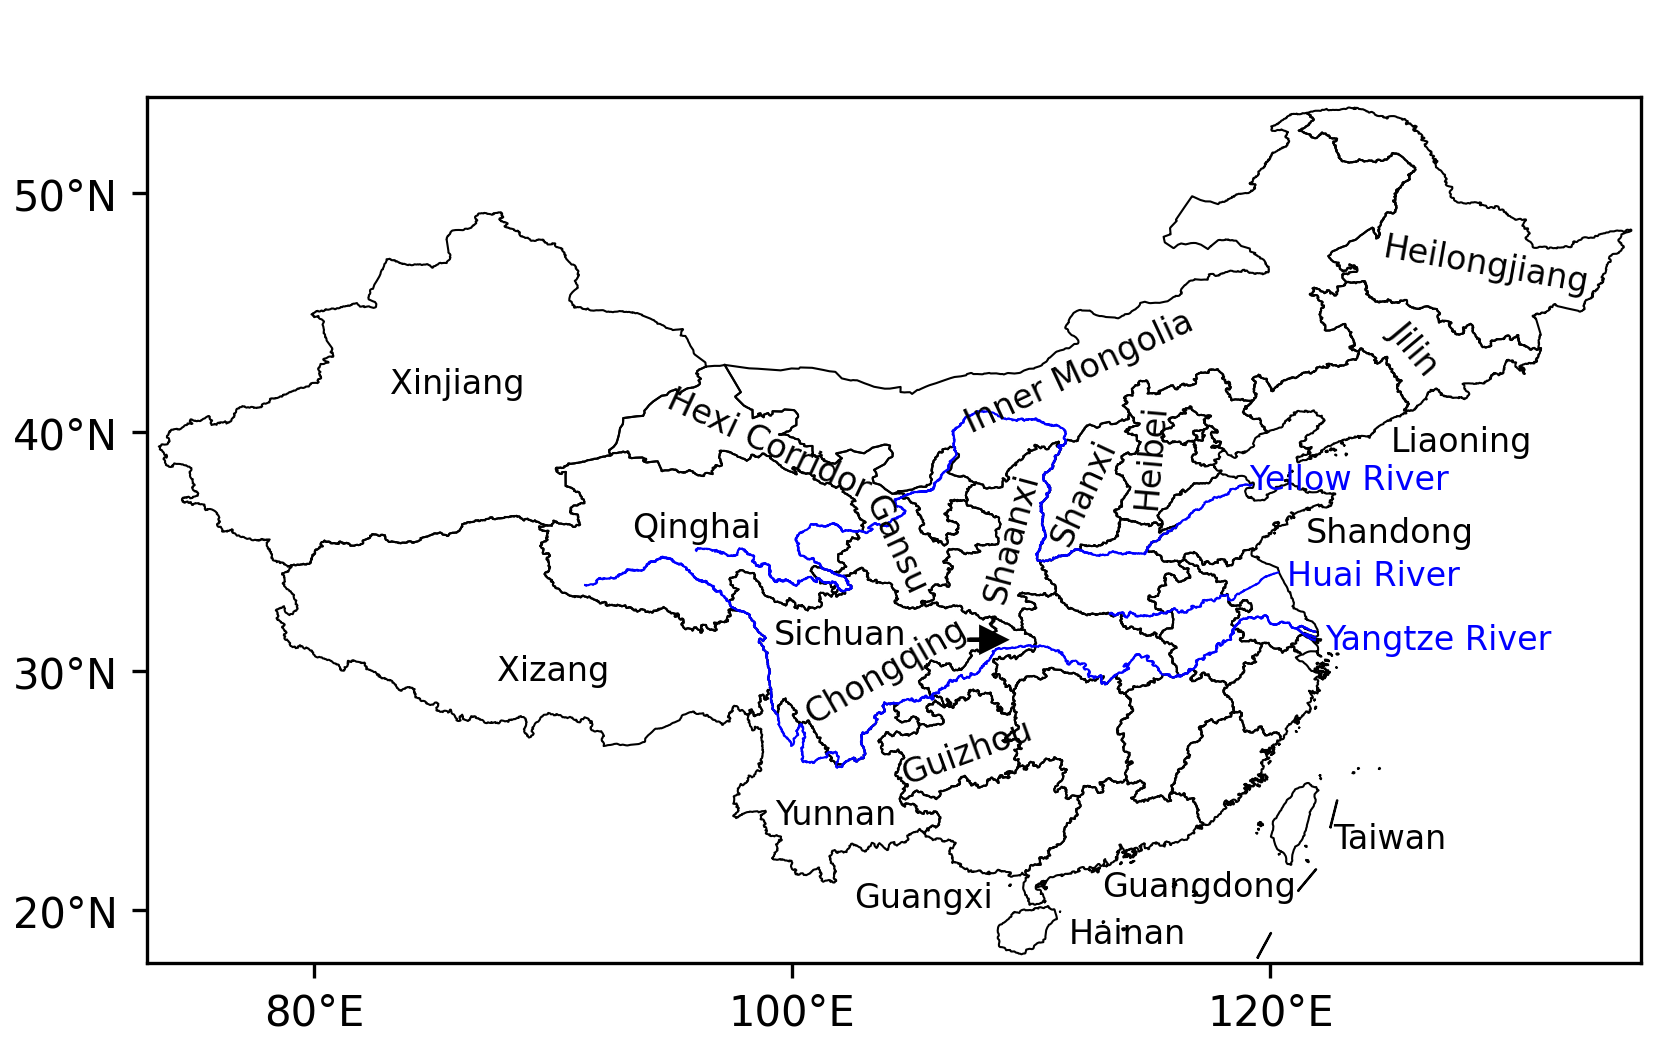
\includegraphics[width=13.8cm]{fig/map.png}
  \caption{Study domain. Blue lines denote the Yangtze and Huai Rivers. Black lines denote the province~boundaries.\label{fig:chinamap}}
\end{figure}
\unskip

\begin{table}[H]
  \caption{Experimental~settings.\label{tab:exp}}
  \newcolumntype{C}{>{\centering\arraybackslash}X}
  \begin{tabularx}{\textwidth}{CCcC}
    \toprule
    \textbf{Experiment} & \textbf{Method} & \textbf{Averaging Weights~\textsuperscript{1}}         & \textbf{Climatology} \\
    \midrule
    A                   & TMY             & 1/2, 1/12, 1/24, 1/24, 1/12, 1/24, 1/24, 1/12, \& 1/12 & 1991--2020           \\
    B                   & TMY             & The same as A                                          & 2011--2020           \\
    C                   & TMY             & The same as A                                          & 2001--2020           \\
    D                   & TMY             & The same as A                                          & 1981--2020           \\
    E                   & TMY             & The same as A                                          & 1971--2020           \\
    F                   & MYA             & -                                                      & 1991--2020           \\
    G                   & TMY             & The same as A                                          & 2011--2020           \\
    H                   & MYA             & -                                                      & 2011--2020           \\
    I                   & TMY             & 12/20, 2/20, 1/20, 1/20, 2/20, 1/20, 1/20, 0, \& 0     & 1991--2020           \\
    J                   & TMY             & 12/20, 2/20, 1/20, 1/20, 0, 0, 0, 2/20, \& 2/20        & 1991--2020           \\
    K                   & TMY             & 12/20, 0, 0, 0, 2/20, 1/20, 1/20, 2/20, \& 2/20        & 1991--2020           \\
    \bottomrule
  \end{tabularx}
  \noindent{\footnotesize{\textsuperscript{1} The averaging weights of the Finkelstein--Schafer statistics for the surface downwelling solar irradiance, 2m air temperature, daily maximum air temperature, daily minimum air temperature, dew point temperature, daily maximum dew point temperature, daily minimum dew point temperature, daily mean wind speed, and~daily maximum wind speed, respectively.}}
\end{table}

\section{Results and~Discussion}\label{sec:results}
\unskip

\subsection{Annual Solar~Radiation}

\Cref{fig:richness_grade} shows the spatial distribution of China's solar energy resources estimated from Experiment~A. The~resources are the most abundant (grade A) in the Tibetan Plateau, southern Xinjiang, western Inner Mongolian Plateau, and~western Sichuan province. These areas occupy 28\% of the whole territory of China. 42\% of China exhibits modest resources (grade B). The~areas are located in northern Xinjiang, the~eastern Inner Mongolian Plateau, eastern Gansu Province, northern Shaanxi Province, and~major parts of Yunnan, Shanxi, Jilin, Liaoning, Hebei, Shandong, Taiwan, and~Hainan. There are 29\% of China that have relatively low resources (grade C). The~areas are mainly located in the middle to lower Yangtze River basin and parts of the Northeast. Meager resources (grade D) are found at the junction of Chongqing and Guizhou, which covers about 1\% of China. The~estimates are generally consistent with previous studies in the places where in situ observations are available~\cite{tang2023ESSD}. In~comparison with the assessment using interpolated in situ data~\cite{li2010PG}, a~lower estimate was found in the Hexi Corridor, where in situ observations are~sparse.

\begin{figure}[H]
  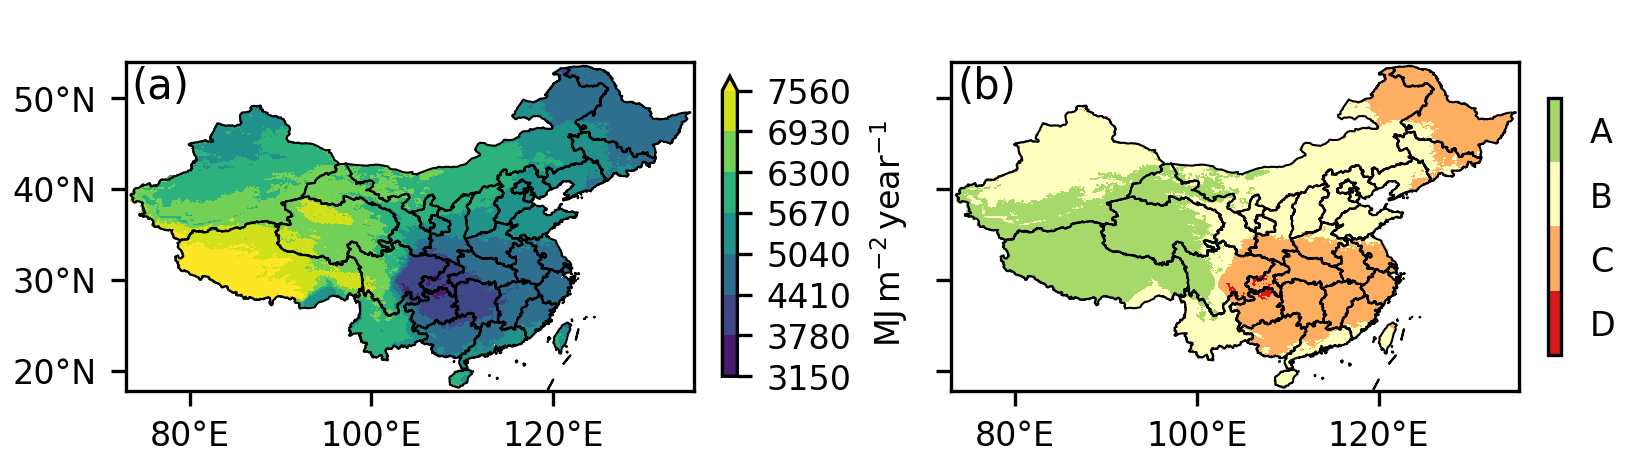
\includegraphics[width=13.8cm]{fig/tmy-resource-grade.png}
  \caption{China's solar energy resources assessed using the TMY method for a thirty-year period (1991 to 2020). (\textbf{a}) annual global horizontal solar radiation, and~(\textbf{b}) abundance grade of the solar energy~resources. The definitions of the grades A, B, C, and D are described in \Cref{sec:datamethods:experiments} \label{fig:richness_grade}}
\end{figure}

\Cref{fig:tmy_length} presents the relative difference between Experiments~B--E to Experiment~A. The~ten-year estimates show a significant difference from the thirty-year ones in most areas of China. The~0.9, 0.95, and~0.99 quantiles of the absolute difference are 3.79\%, 4.59\%, and~6.55\%, respectively. The~significant discrepancy suggests that ten years may not be sufficiently long to assess solar energy resources. The~longer the data records, the~more stable the assessment. The~twenty-year estimates are closer to the thirty-year estimates. The~0.9, 0.95, and~0.99 quantiles are reduced to 3.05\%, 3.64\%, and~4.90\%, respectively. A~longer period beyond 30 years yields marginal differences. The~0.9, 0.95, and~0.99 quantiles of the absolute difference between the thirty-year and forty-year estimates are 2.18\%, 2.70\%, and~3.83\%, respectively. These values are almost half of those for the ten-year estimates. The~marginal difference suggests that a thirty-year period is sufficient for the assessment. Interestingly, the~fifty-year estimates show a larger deviation than the forty-year estimates. We speculate that the deviation is due to the inhomogeneity of the CMFD data before 1981. This period has few in situ observations and almost zero satellite observations to correct the biases in ERA5\@. Therefore, we focus on the thirty-year period from 1991 to 2020 (Experiment~A) in the following~analyses.

\Cref{fig:tmy_mya_diff_mean} compares Experiment~A versus F and Experiment~G versus H. The~comparisons reveal the difference between the TMY and MYA methods in estimating the annual total solar radiation. The~probability distribution function of the differences is symmetric around zero. The~absolute relative difference estimated using the thirty-year data from 1991 to 2020 is less than 2.69 (the 0.99 quantiles), with~a median value of 0.6\%. The~difference is mainly exhibited in parts of Shaanxi, eastern Sichuan, Chongqing, and~Guizhou, where the Southwest China vortex and topographic effects have a strong influence. The~difference between the TMY and MYA methods does not show a strong dependency on the reference period length. The~median value of the absolute difference is 0.6\% for the 30 years (\mbox{\Cref{fig:tmy_mya_diff_mean}b}) and 0.7\% for the 10 years (\Cref{fig:tmy_mya_diff_mean}d). However, the~locations of the difference vary with the selection of the reference period. For~the 10 years, from~2011 to 2020, in~addition to the regions listed above, the~lower Yangtze River basin, Guangxi, and~parts of Heilongjiang also exhibited changes. The~spatial distributions hint at the influence of the East Asia monsoon and the northeast China cold vortex. Despite the difference described above, the~TMY and MYA methods are indistinguishable in classifying the solar energy resource abundance grade, with~only 3.5\% area of China having a different grade (1.85\% for upgrade and 1.68\% for downgrade).

\begin{figure}[H]
  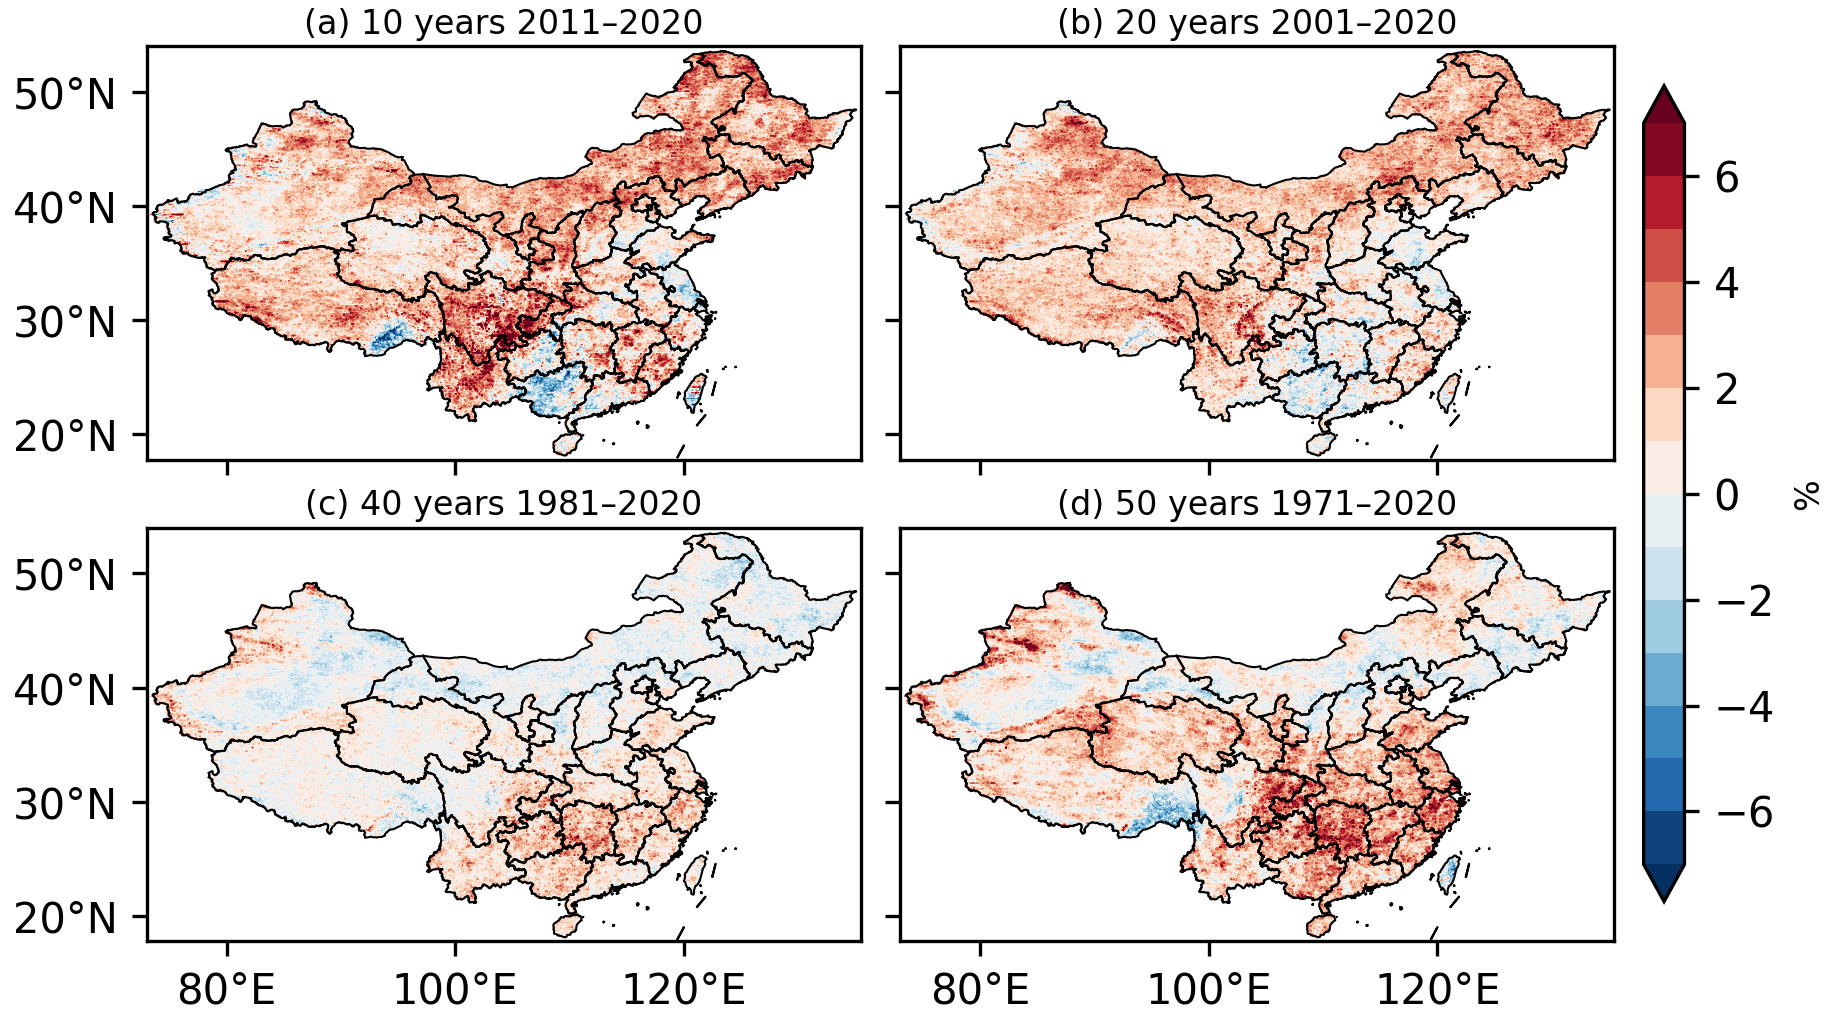
\includegraphics[width=13.8cm]{fig/tmy-change-datalength.png}
  \caption{Relative changes in the solar radiation estimates using the reference periods of different lengths. The~changes are relative to the thirty-year period from 1991 to 2020\@: (\textbf{a}) 10 years from 2011 to 2020; (\textbf{b}) 20 years from 2001 to 2020; (\textbf{c}) 40 years from 1981 to 2020; and~(\textbf{d}) 50 years from 1971 to~2020.\label{fig:tmy_length}}
\end{figure}
\vspace{-6pt}

\begin{figure}[H]
  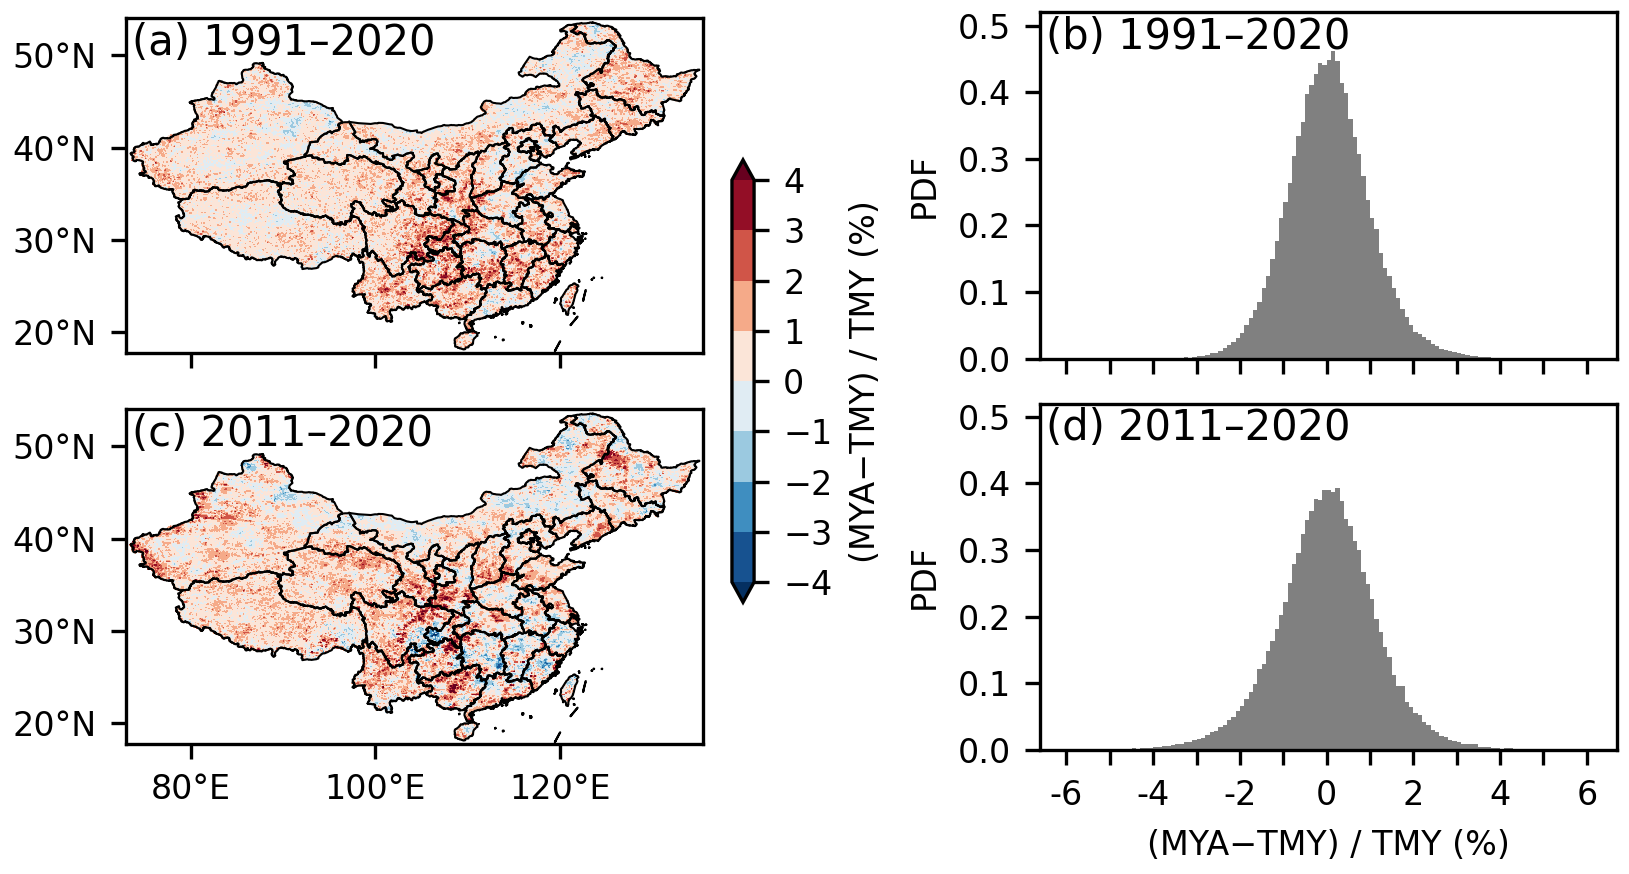
\includegraphics[width=13.8cm]{fig/mya-tmy-diff-hist.png}
  \caption{Relative difference between the MYA and TMY methods in calculating annual solar radiation. The~left panels present the spatial distribution, whereas the right panels present the probability distribution function (PDF).\label{fig:tmy_mya_diff_mean}}
\end{figure}
\unskip

\subsection{Seasonal~Variations}

\Cref{fig:seasonal_fraction} shows the seasonal solar radiation estimated from Experiment~A. The~seasonal radiation is presented as a fraction of the annual total for comparing values at different places across China. The~radiation is largest in summer and smallest in winter. Across the whole study domain, the~middle Yangtze River basin and the northern parts of northeast China, Inner Mongolia, and~Xinjiang exhibit the highest radiation in summer and the lowest radiation in winter. In~autumn, the~fraction is nearly uniform, except~for a slightly higher value in Guangdong and Guangxi and a marginally lower one in the northern part of northeast China. In~spring, northern China shows a slightly higher seasonal fraction than southern~China.

\begin{figure}[H]
  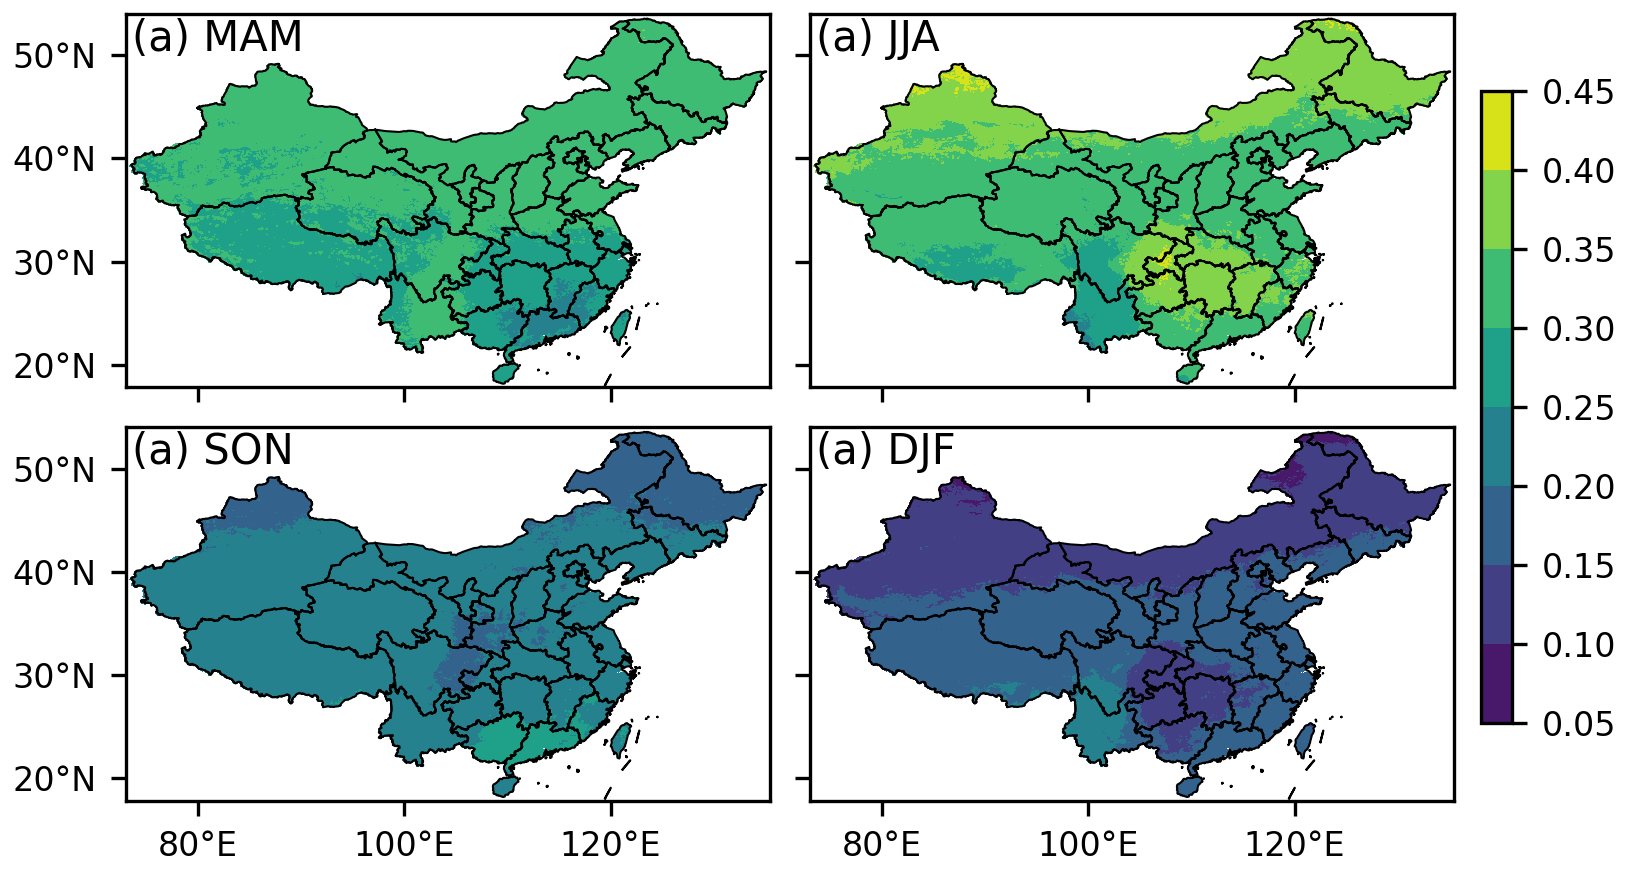
\includegraphics[width=13.8cm]{fig/tmy-seasonal-fraction.png}
  \caption{Seasonal radiation estimated with the TMY method for the thirty-year period (1991 to 2020). The~values are fractions of the annual totals. (\textbf{a}) MAM for March, April, and~May; (\textbf{b}) JJA for June, July, and~August; (\textbf{c}) SON for September, October, and~November; and (\textbf{d}) DJF for December, January, and~February. \label{fig:seasonal_fraction}}
\end{figure}

\Cref{fig:stability_grade} classifies the seasonal stability grade based on the seasonal radiation fraction shown in \Cref{fig:seasonal_fraction}. The~stability grade is highest in Yunnan, western Sichuan, and~southern Xizang. The~areas where the winter-to-summer radiation ratio is above 0.47 (grade A) cover 19.29\% of China. The~stability grade is lowest in the Northeast, eastern Inner Mongolia, and~northern Xinjiang. The~winter-to-summer radiation ratio is below 0.28 in these areas, and~they cover 20.03\% of China. The~other areas have moderate stability. In~these areas, the~northern parts generally have higher seasonal stability than the southern ones. The~areas with grade B and grade C stabilities cover 30.47\% and 29.82\% of \mbox{China, respectively.}

\begin{figure}[H]
  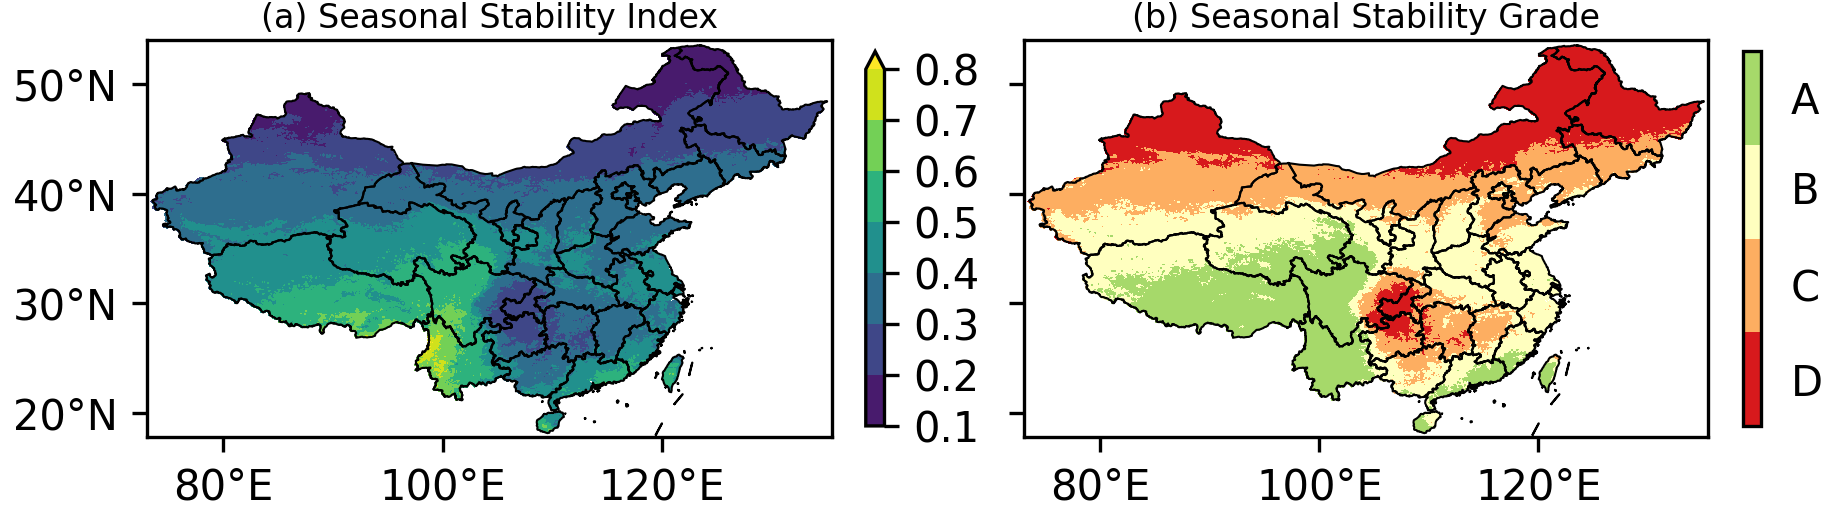
\includegraphics[width=13.8cm]{fig/tmy-seasonal-stability-index-grade.png}
  \caption{Seasonal stability index and grade of the solar energy resource assessed using the TMY method for the thirty-year period (1991 to 2020). The~seasonal stability index is defined as the ratio of the minimum monthly radiation to its maximum~value. The stability grades A, B, C, and D are defined in \Cref{sec:datamethods:experiments}. \label{fig:stability_grade}}
\end{figure}

\Cref{fig:tmy_mya_diff_sea} shows the seasonal radiation difference between the TMY and MYA methods (i.e., Experiment~A versus F). The~difference is larger in spring and summer. The~range of the absolute difference measured by the 0.99 quantile is 1.44\% of the annual total in spring and 1.58\% in summer. Autumn and winter show a relatively smaller difference, with~a 0.99 quantile of 1.16\% and 1.00\%, respectively. The~seasonal variations in the difference between the TMY and MYA methods reflect the activity of weather systems. Relatively active weather systems in summer increase the difference, whereas the difference is reduced in winter due to relatively stable weather conditions. The~area with a notable seasonal difference coincides with the area with the abundance grade of C (\Cref{fig:richness_grade}b), which is the middle and lower Yangtze River basins, the~middle Yellow River basin, the~Huaihe River basin, and~northeast China. Northern China exhibits a slightly seasonal dependency. The~difference in northeast China is notable in spring and summer but diminishes in winter. This seasonal variation in southern China is much weaker. The~middle and lower Yangtze River basins are the areas with the most notable differences all year round. Unlike the difference in the annual total (\Cref{fig:tmy_mya_diff_mean}), the~difference in the seasonal radiation is skewed around zero, and~the skewness varies with season. MYA tends to have a slightly lower estimate in summer and a marginally higher estimate in spring than TMY\@. The~median difference is \textminus{}0.011\% and 0.029\% for summer and spring, respectively.

\begin{figure}[H]
  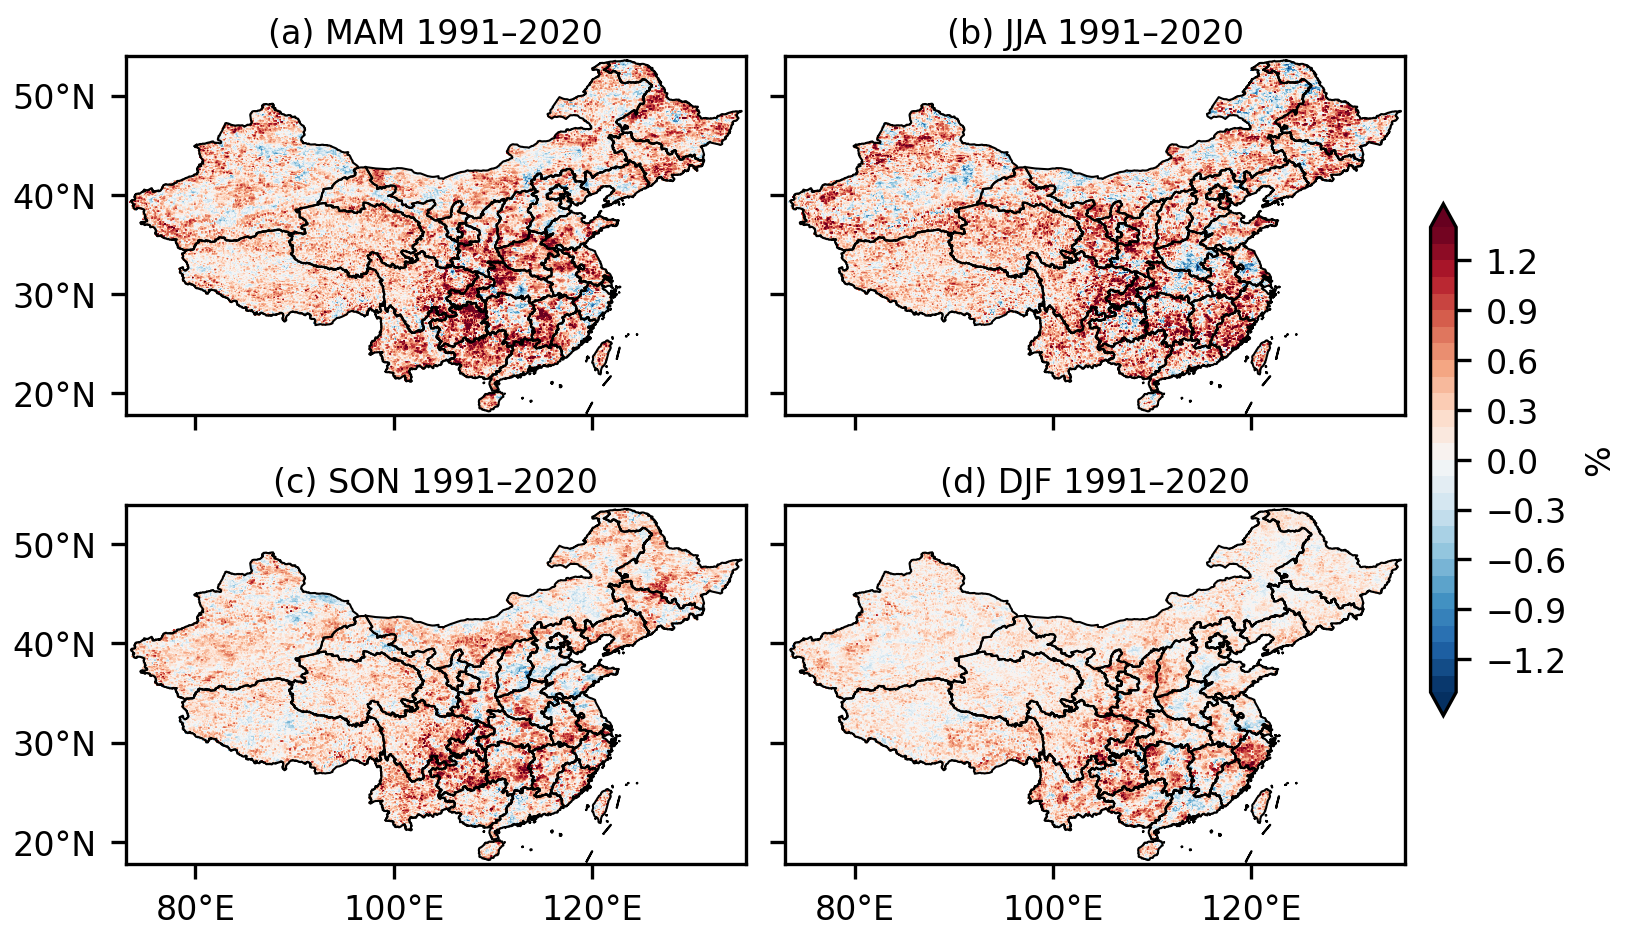
\includegraphics[width=13.8cm]{fig/mya-tmy-seasonal-30yr.png}
  \caption{Difference between the MYA and TMY methods in calculating seasonal solar radiation for the thirty-year reference period (1991 to 2020). The~values are presented as the percentage of the annual solar radiation estimated using the TMY method (\Cref{fig:richness_grade}a). \label{fig:tmy_mya_diff_sea}}
\end{figure}

\Cref{fig:stability_tmy_mya_diff} shows the difference in the stability index and grade between the TMY and MYA methods (i.e., Experiment~A versus F). Consistent with the discussion above, the~probability distribution function of the difference in the stability index is slightly skewed to the right, indicating that the MYA method tends to have a higher stability index than the TMY. The~difference is more notable in southwestern China, including Yunnan, Sichuan, Guangdong, and~Guangxi. The~increase in the stability index is consistent with the lower summer and higher winter radiation, as~shown in \Cref{fig:tmy_mya_diff_sea}. The~difference in the seasonal stability grade is more notable compared with the annual total. A total of 10.5\% of China has a different stability grade. Approximately 70\% of these areas experience an upgrade, whereas the other 30\% experience a~downgrade.

\begin{figure}[H]
  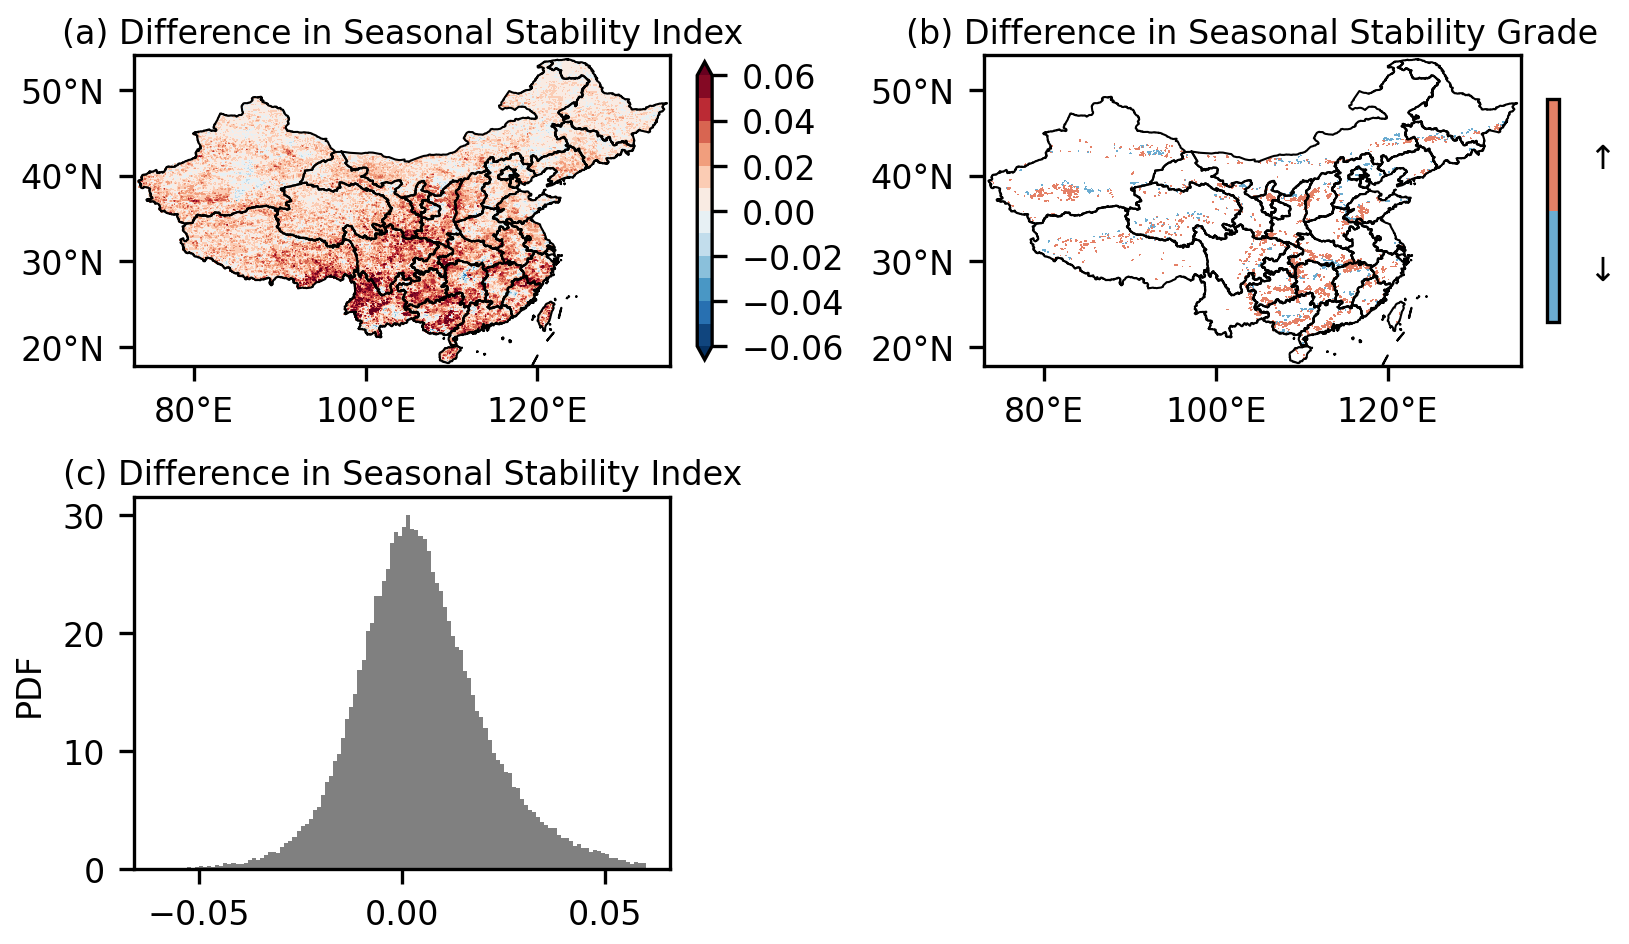
\includegraphics[width=13.8cm]{fig/mya-seasonal-stability-index-grade.png}
  \caption{Difference in the seasonal stability index and grade between the MYA and TMY methods: (\textbf{a}) Difference of the MYA method relative to TMY; (\textbf{b}) Difference in the seasonal stability grade of the MYA method relative to TMY. Red denotes an upgrade (up arrow), whereas blue denotes a downgrade (down arrow); \mbox{(\textbf{c}) Probability} distribution function (PDF) of the difference in the seasonal stability~index.\label{fig:stability_tmy_mya_diff}}
\end{figure}
\unskip

\subsection{Impacts of the Meteorological~Variables}

\Cref{fig:tmy_ann_var_sens} shows the difference between Experimnents~I, J, and~K to Experiment~A. The~difference delineates the impact of the meteorological variables on estimating the annual solar radiation. The~impacts are marginally smaller than the difference between the TMY and MYA methods (\Cref{fig:tmy_mya_diff_mean}). The~0.99 quantiles of the absolute difference are 2.71\%, 2.41\%, and~2.57\% of the annual total for wind speed, air temperature, and~dew point, respectively. Wind speed generally has the most considerable impact among the three variables, with~a median absolute difference of 1.85\% of the annual total. The~dew point has the second most considerable impact. The~median absolute difference is 1.77\% of the annual total. The~air temperature makes the smallest difference with a median value of 1.68\%. The~three variables have similar patterns of impact. The~impacts are more notable in northeast China and the middle Yangtze River basin, which have low solar energy resources (grades B and C as shown in \Cref{fig:richness_grade}). The~impacts of wind speed and dew point tend to have an opposite direction. Consideration of the wind speed slightly decreases the estimate (0.013\% of the annual total in median), whereas consideration of the air temperature and dew point slightly increases the estimate (0.011\% of the annual total in median).

\Cref{fig:tmy_sea_var_sens} is the same as \Cref{fig:tmy_ann_var_sens} but for the seasonal stability index. The~impacts are all symmetric around zero for the three variables. Like the annual total as shown in \Cref{fig:tmy_ann_var_sens}, the~wind speed has the most considerable impact, the~air temperature has the least significant effect, and~the dew point lies in between. The~range of the impacts measured by 0.99 quantiles of the absolute difference is similar for the three variables, which are 0.57 for wind speed, 0.054 for air temperature, and~0.054 for dew point. However, the~median absolute difference is slightly larger for wind speed (0.035) than for temperature (0.032) and dew point (0.033). Unlike the annual total, the~seasonal stability index's changes are clustered only in the middle to lower Yangtze River basin and are negligible in the~Northeast.

\begin{figure}[H]
  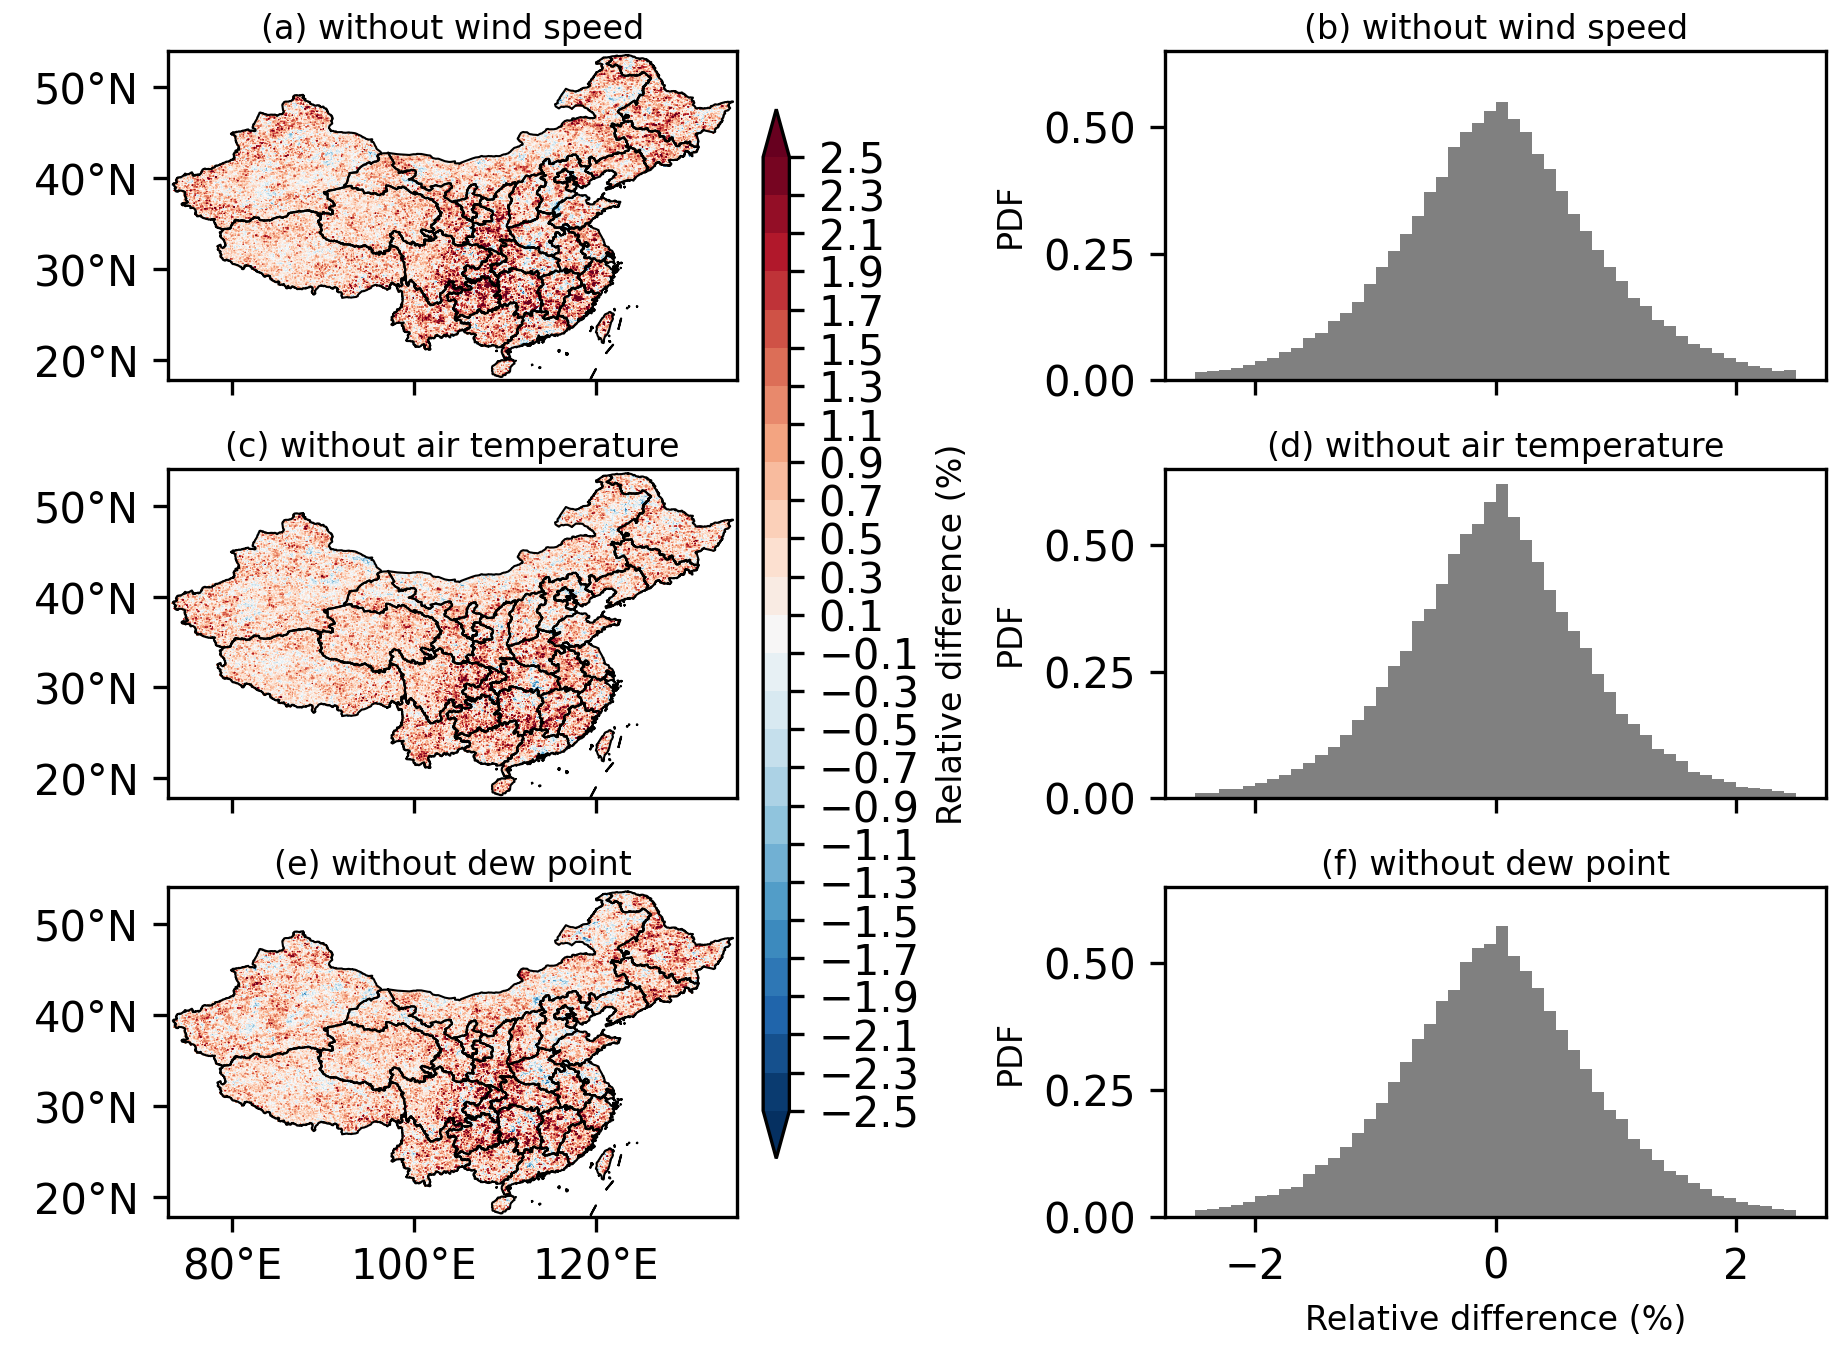
\includegraphics[width=13.8cm]{fig/tmy-ann-var-sensitivity.png}
  \caption{Sensitivity of annual solar radiation to the considered meteorological variables. The three rows present the impacts of wind speed, air temperature, and dew point, respectively. The~right panels present the probability distribution function of the relative differences corresponding to the left~panels.\label{fig:tmy_ann_var_sens}}
\end{figure}
\vspace{-6pt}

\begin{figure}[H]
  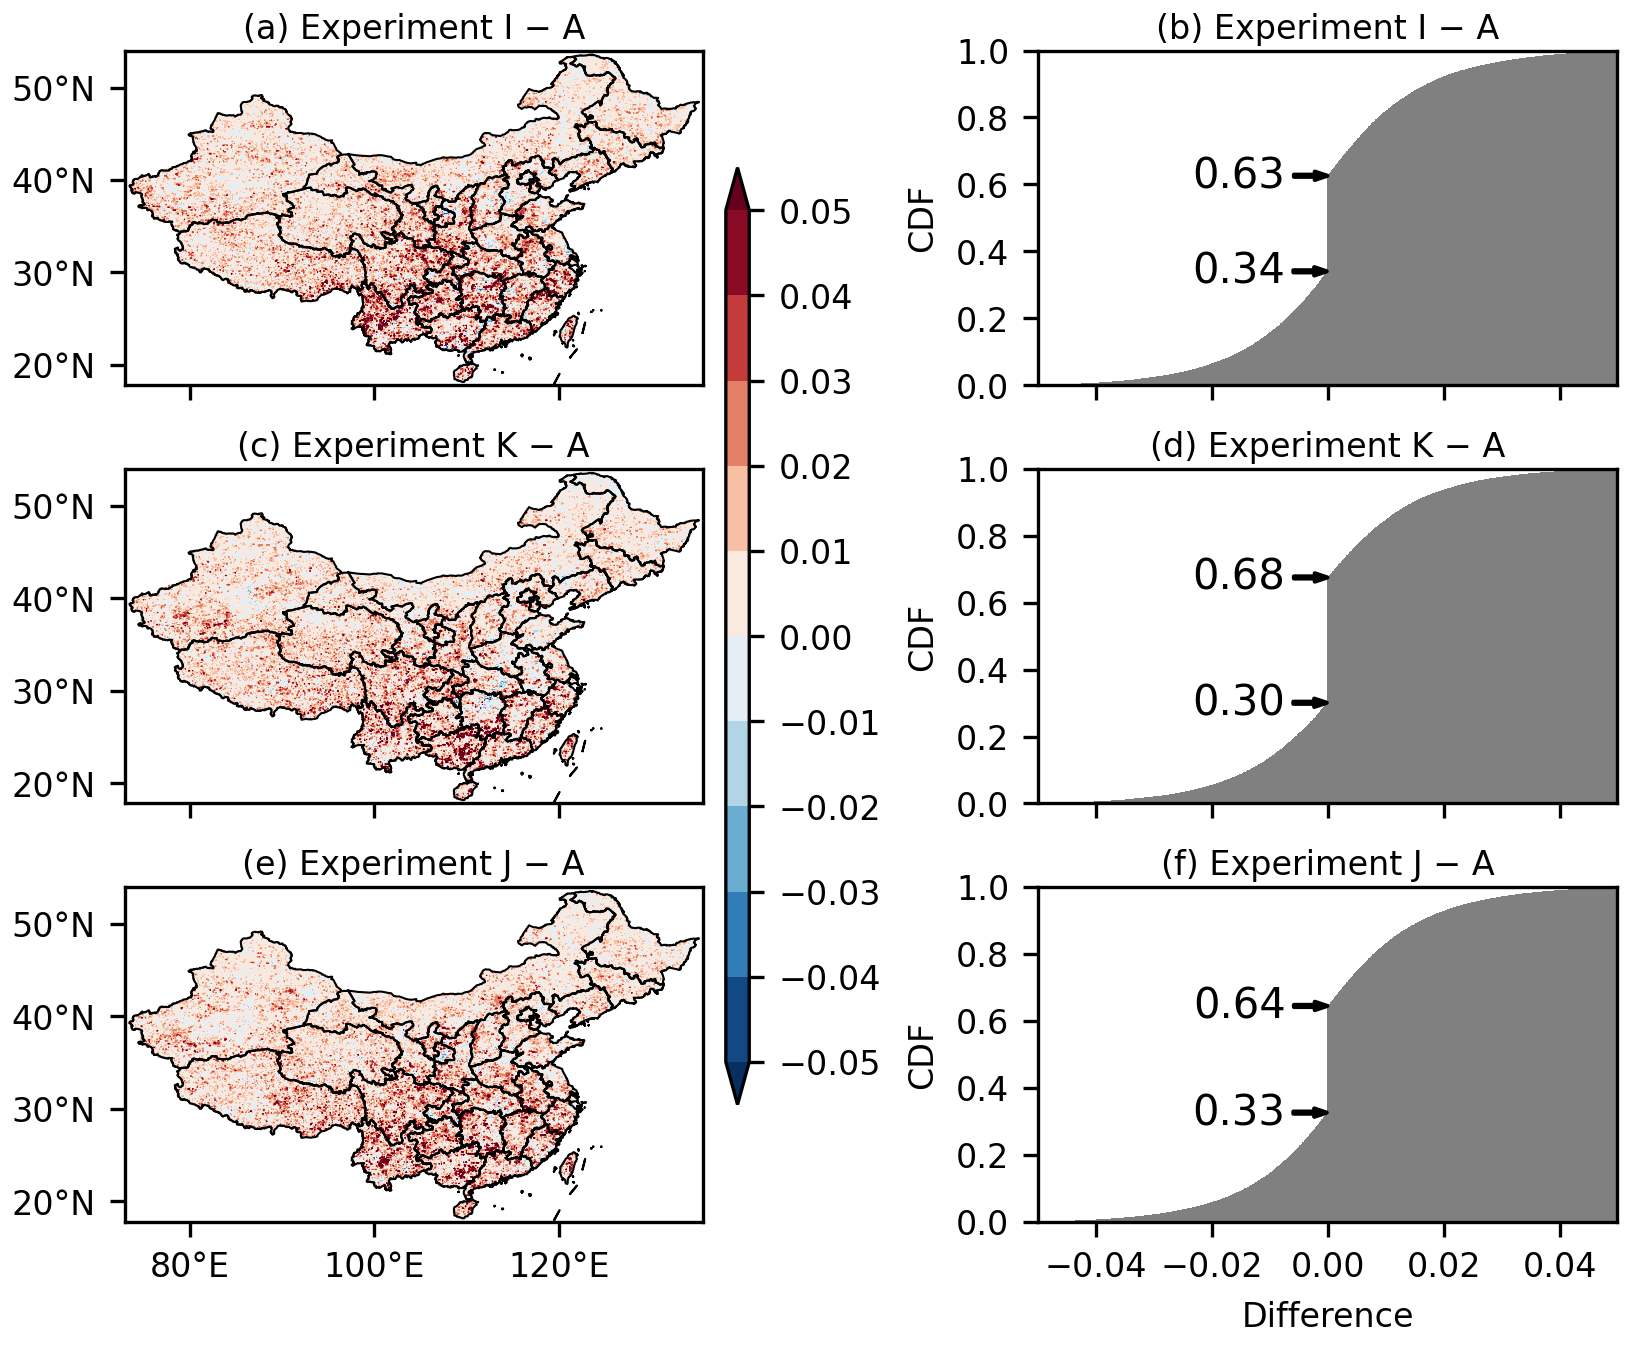
\includegraphics[width=13.8cm]{fig/tmy-sea-var-sensitivity.png}
  \caption{Sensitivity of the seasonal stability index to the considered meteorological variables. The three rows present the impacts of wind speed, air temperature, and dew point, respectively. The~right panels present the cumulative distribution function of the relative changes corresponding to the left panels. The~lower and upper numbers in the right panels denote the CDFs of the area with negative and non-negative changes, respectively. \label{fig:tmy_sea_var_sens}}
\end{figure}
\unskip

\section{Conclusions}\label{sec:conclusions}

This study delineated the solar energy resources of mainland China using the TMY method and the CMFD dataset and the impacts from the records lengths in various reference periods. The~areas with the abundance grades A, B, C, and~D cover 28\%, 42\%, 29\%, and~1\% of the whole territory of China, respectively. The~annual total solar radiation is most abundant (grade A) in the Tibetan Plateau, southern Xinjiang, and~the Inner Mongolian Plateau. The~solar energy resources are low (grace C or D) in the northeastern part of northeast China, the~middle to lower Yangtze River basin. The~other regions fall in between. The~longer the data records, the~more stable the assessment. The~assessments become acceptably stable using data records that are equal to or longer than 30~years.

This study compared the TMY and MYA methods. Their differences in the annual total are symmetric around zero. The~difference is mainly exhibited in Yunnan, Sichuan, Guangdong, Guangxi, and~Shaanxi. The~difference is nearly invariant with the data record length, hinting at the location-specific long-term weather characteristics. The~differences in the seasonal stability index are more notable. The~stability grade differs in approximately 10.5\% of China. The~region is mostly the same as that for the annual total. The~difference in the seasonal stability is skewed. Among~these regions with different stability grades, approximately 70\% experience a downgrade from TMY, whereas the other 30\% experience an upgrade. In~these mentioned provinces, an~assessment method that can consider weather characteristics (e.g., TMY) is~preferred.

This study also revealed the impact of three meteorological variables (i.e., wind speed, air temperature, and~dew point) on the TMY-based assessment. Wind speed generally has the most considerable impact, air temperature has the least significant effect, and~dew point lies in between. The~difference is notable in places with modest solar energy resources where the weather conditions are the most variable. The~spatial pattern of the difference varies with the variables. All three variables exhibit different annual total and seasonal stability in the middle to lower Yangtze River basin; whereas, in~the Northeast, the~impact of air temperature is~negligible.

The results suggest that weather conditions have notable impacts on the solar energy abundance and seasonal variations in southwest China. However, the~region tends to have significant data uncertainty due to relatively limited in situ observations and complex topography. Future assessments based on satellite observations and high-resolution model simulations would be helpful to reduce~uncertainty.

\vspace{6pt}

\authorcontributions{Conceptualization, H.Z.; methodology, H.Z.; data curation, H.Z.; investigation, Z.S.; formal analysis, Z.S.; visualization, Z.S., B.W.; Writing---original draft, Z.S., B.W., S.J., X.L., S.H.; Writing---review \& editing, H.Z.; supervision, H.Z.; project administration, Z.S.; funding acquisition, Z.S.; All authors have read and agreed to the published version of the~manuscript.}

\funding{
  This research was funded by the Science and Technology Project ``The Research of Mechanism and Simulation on the Interaction between the Local Climate and Large-scale Renewable Energy Development'' (Grant No.\ 4000-202155465A-0-0-00) of State Grid Corporation of China (SGCC).
}

\institutionalreview{Not applicable.}

\informedconsent{Not applicable.}

\dataavailability{
  The CMFD version 1.7 used in this study was provided by Dr.\ Jie He at the Institute of Tibetan Plateau Research, Chinese Academy of Sciences. Earlier versions of CMFD are downloadable at \url{https://doi.org/10.11888/AtmosphericPhysics.tpe.249369.file} (accessed on 14 November 2023). The solar radiation data from each experiment and the plotting scripts used in this study are available at \url{https://github.com/hzheng88/paper-2024-china-solar-tmy-cmfd}.
}

\acknowledgments{
  We sincerely thank Jie He at the Institute of Tibetan Plateau Research for his kindness in providing the latest CMFD\@.
}

\conflictsofinterest{Zongpeng Song, Bo Wang, Shuanglong Jin, Xiaolin Liu, and Shenbing Hua are employees of the China Electric Power Research Institute. The paper reflects the views of the scientists and not the company.}
\vspace{+40pt}

% %%
\begin{adjustwidth}{-\extralength}{0cm}
  %\printendnotes[custom] % Un-comment to print a list of endnotes

  % References
  \reftitle{References}
  \bibliography{references.bib}

  \PublishersNote{}
\end{adjustwidth}
\end{document}

%%% Local Variables:
%%% TeX-master: "main"
%%% TeX-engine: default
%%% End:
